\section{App - iOS}
Um möglichst viele Endnutzer für unser Produkt zu erreichen, war es uns wichtig, für die zwei verbreitetsten Smartphone Betriebssysteme Apps bereitzustellen. Für die Entwicklung der iOS-App wurde die Sprache SwiftUI unter Nutzung der  kostenlosen IDE Xcode genutzt.  Da es sich hier um neues Terrain handelte, wurde mehr Zeit zur Einarbeitung und späteren Problemfindung benötigt, als anfänglich gedacht, weshalb diese App eher einem Design-Prototypen entspricht. 

\subsection{Xcode}
Mit Xcode können Programme für macOS, iPadOS, iOS, watchOS und tvOS entwickelt werden. Diese IDE ist für die Programmiersprachen Swift und Objective-C unter Verwendung der Cocoa-Frameworks vorgesehen, wobei aber auch die Programmiersprachen C und C++ verwendet werden können. Aufgrund seiner Modularität ist es jedoch auch möglich Programme in anderen Sprachen zu schreiben – beispielsweise in Java, Ruby, Perl oder Pascal. \cite{Ahmad2020}
\\
\\
Wie von Apple gewohnt, bietet Xcode eine übersichtliche wie aufgeräumte Benutzeroberfläche. Beim Starten eines neuen Projektes hilft ein Assistent bei den richtigen Einstellungen. Neben dem Programmieren von Apps unterstützt das Tool auch das visuelle Gestalten der späteren Benutzeroberfläche sowie das Testen und Debuggen von Software. \cite{Ahmad2020}
\\
\\
Die IDE kommt mit einem grafischen Interface-Design-Tool namens Interface Builder, über das Benutzeroberflächen entwickelt werden können. Menüs, Fenster, Controls und weitere visuelle Elemente lassen sich gestalten oder aus vorhandenen Objekten, aus einer integrierten Bibliothek ziehen. Alternativ können natürlich auch eigene entwickelt werden. Die Anbindung bestimmter Elemente an den dahinterliegenden Code (\textit{in Form von ausführbaren Aktionen beispielsweise}) ist mit dem Interface Builder ebenfalls möglich.\cite{Ahmad2020}
\\
\\
Für Xcode wurde sich einerseits entschieden, um später keine Komplikationen mit der Kompatibilität auf dem Endgerät zu riskieren. Bei der Recherche, welche IDE wir nutzen möchten, wurde relativ schnell klar, dass dies bei anderen kostenlosen IDE Tools passieren könnte. Andererseits überzeugten die vielen hinterlegten Simulatoren - von iPad, über Macbook bis hin zu sämtlichen iPhone Generationen ist alles dabei - welche ein Arbeiten mit schnellem Feedback auf unterschiedlichen Geräten ermöglichen, ohne diese physisch Zuhause haben zu müssen.

\subsection{SwiftUI}
Bei SwiftUI handelt es sich um ein GUI-Framework aus dem Hause Apple, welches auf MVVM\footnote{Model View ViewModel = ein Entwurfsmuster, zur Trennung von Darstellung und Logik der UI} basiert.
Es bietet Ansichten, Steuerelemente und Layoutstrukturen zum Deklarieren der Benutzeroberfläche einer App. Das Framework bietet Event-Handler für die Bereitstellung von Taps, Gesten und anderen Arten von Eingaben an der App sowie Tools zur Verwaltung des Datenflusses von den Modellen der App bis hin zu den Ansichten und Steuerelementen, die Benutzer sehen und mit denen sie interagieren.\cite{Inca}
\\
\\
Die App-Struktur wird mithilfe des App-Protokolls definiert und füllt sie mit Szenen, welche die Ansichten enthalten, aus denen die Benutzeroberfläche der entstehenden App besteht. Es können eigene benutzerdefinierte Ansichten erstellt werden, die dem Ansichtsprotokoll entsprechen, sowie  SwiftUI-Ansichten zum Anzeigen von Text, Bildern und benutzerdefinierten Formen mithilfe von Stapeln, Listen und mehr. \cite{Inca}

\subsection{Hauptkriterien an die Funktionalität}

Damit die App erkennt, ob sich das Auto bewegt oder nicht, muss sie mit dem Webserver kommunizieren können, um sich dort die vom Arduino gesendeten GPS-Daten zu holen. Zusätzlich muss eine Logik implementiert werden, welche bei eingeschaltetem System eine Veränderung der GPS-Daten erkennt und der Nutzer eine Benachrichtigung erhält. Weiterhin benötigen wir eine Funktion, dass die Koordinaten  nicht als plain-Text angezeigt werden, sondern direkt auf einer Karte, wie man es beispielsweise von Google Maps gewohnt ist. Eine weitere sinnvolle  aber eher optionale Implementierung wäre es, wenn die App erkennt, ob der Server gerade erreichbar ist und ein Icon dementsprechend die Farbe ändert.  Um die theoretischen Prozesse zu strukturieren und auch übersichtlich zu visualisieren, haben wir über das Tool Camunda einen ersten groben Ablaufplan erstellt, wie in Abbildung \ref{camunda} zu sehen.


\begin{figure} [H]
	\begin{center}
		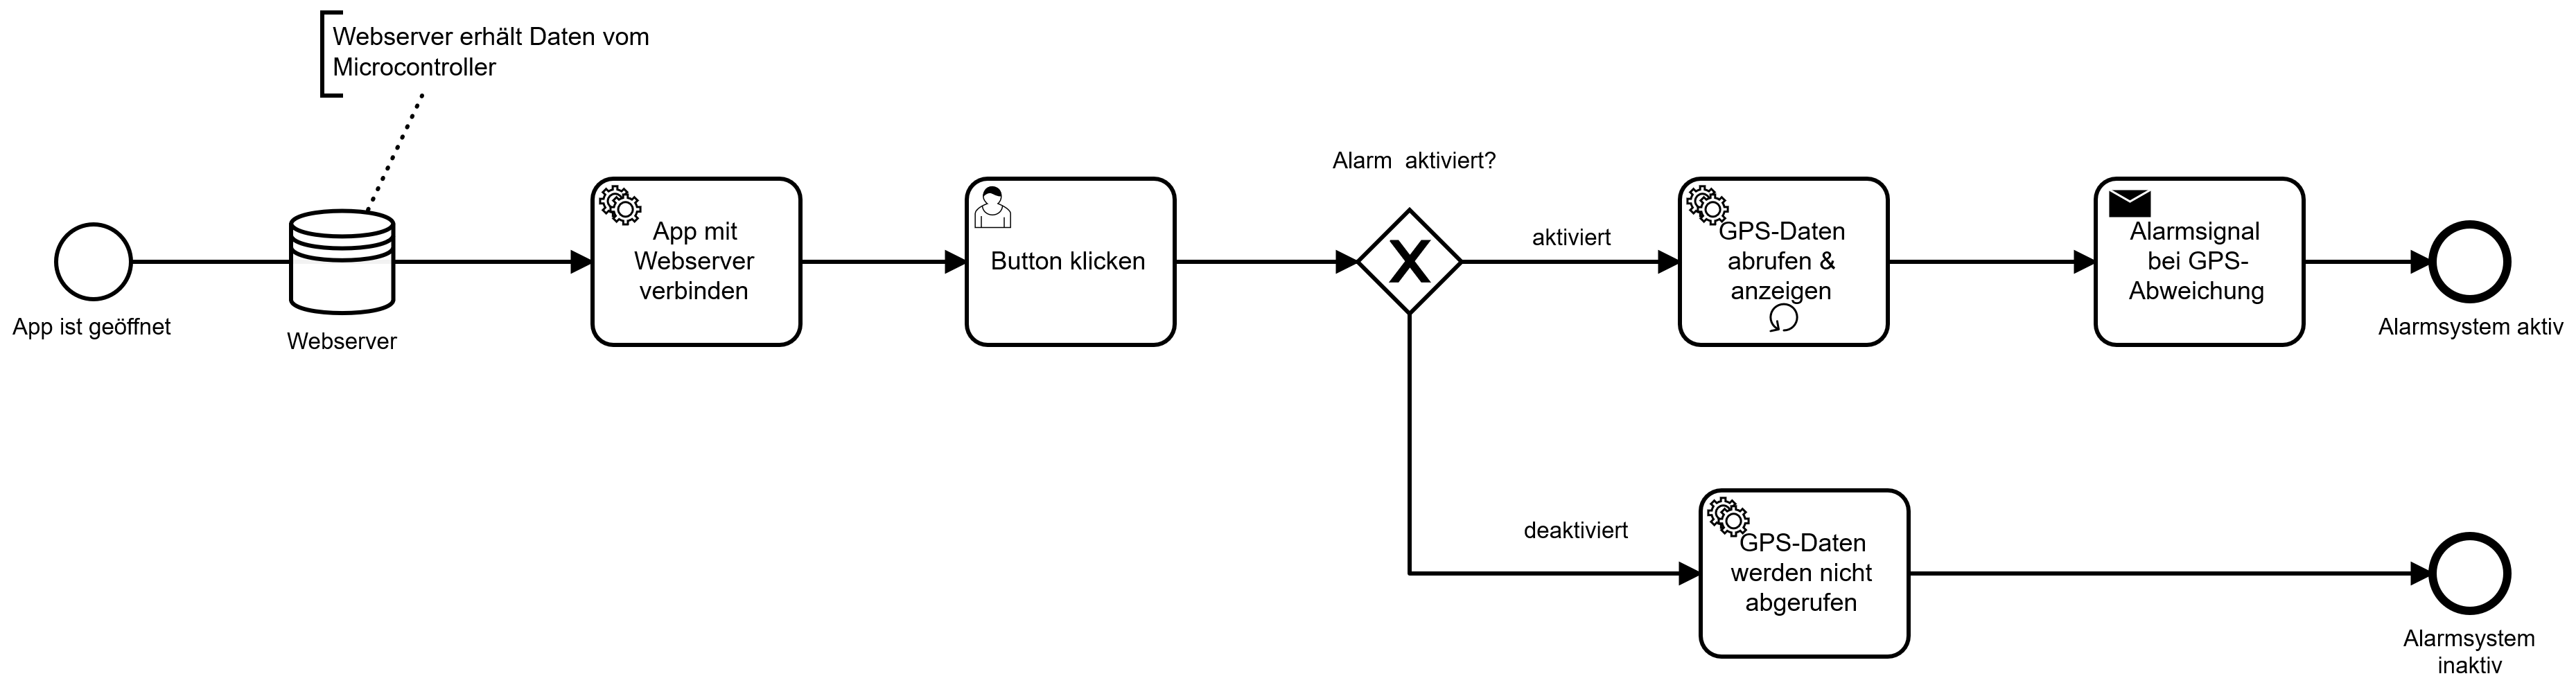
\includegraphics[width=1\textwidth]{Bilder/iOS_camunda.png}
		\caption{Entwurf der Hauptfunktionalitäten}
		\label{camunda}
	\end{center}
\end{figure}
\clearpage

\subsection{Design}
Das Design der beiden Apps unterscheidet sich stark und das wurde auch bewusst von uns zugelassen - es war uns wichtig, Hauptkriterien der Funktionalitäten zu definieren, wie beispielsweise in Abbildung \ref{camunda} zu sehen, aber der Kreativität jedes einzelnen von uns wollten wir keine Grenzen vorschreiben.
\\
\begin{center}
	\textit{Kreativ werden wir dann, wenn wir unsere immer gleichen Muster, unsere üblichen Gedankenabläufe unterbrechen und unseren Geist auf ungewohnte Wege schicken}\footcite{Bode2022}
\end{center}
Der Stil dieser App, besticht durch sein sehr minimalistisches und dennoch durch moderne Farben geprägtes Design. Wir haben hierbei auf Intuitivität geachtet und auf  \textit{viel Text} verzichtet, da die App so keine möglichen Sprachbarrieren aufwirft und zeitgemäßer wirkt.
\\
\\
Unscheinbar aber wichtig! Der Nutzer sieht als erstes das AppIcon im Appstore sowie später auf seinem Bildschirm. Hierbei wollten wir erreichen, dass dieses Icon nicht nur zu unserem Produkt passt, sondern auch optisch sehr anspricht. Daher haben wir uns für ein Icon entschieden, welches die Farben der iOS-App enthält sowie ein Auto, wie in Abbildung \ref{AppIcon}  demonstriert.
\begin{figure} [H]
	\begin{center}
		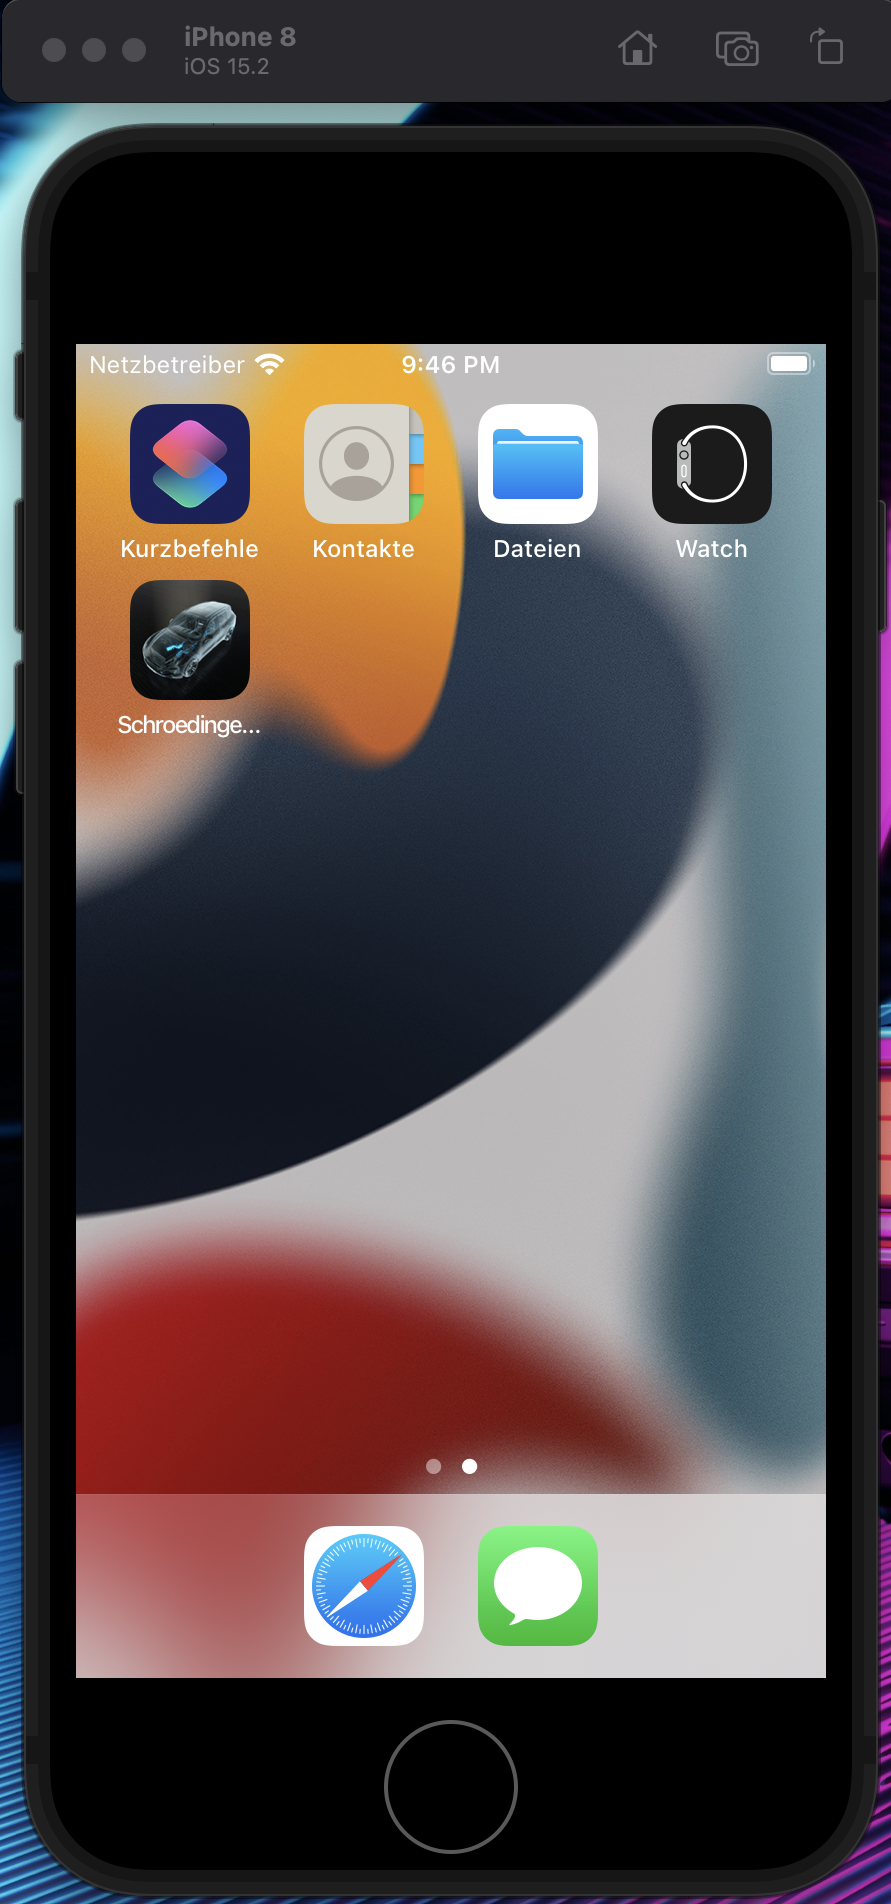
\includegraphics[width=0.4\textwidth]{Bilder/iOS_icon.png}
		\caption{AppIcon auf dem Bildschirm}
		\label{AppIcon}
	\end{center}
\end{figure}
Nach dem berühmten Tap auf das Icon hängt es oftmals vom Alter des genutzten Gerätes ab, wie schnell eine App sich aufbaut. Damit auch hier der User ein Feedback erhält, ob  etwas passiert, haben wir einen Launchscreen implementiert, welcher ebenfalls dem Design der App entspricht.(Abbildung \ref{Launch})
\begin{figure} [H]
	\begin{center}
		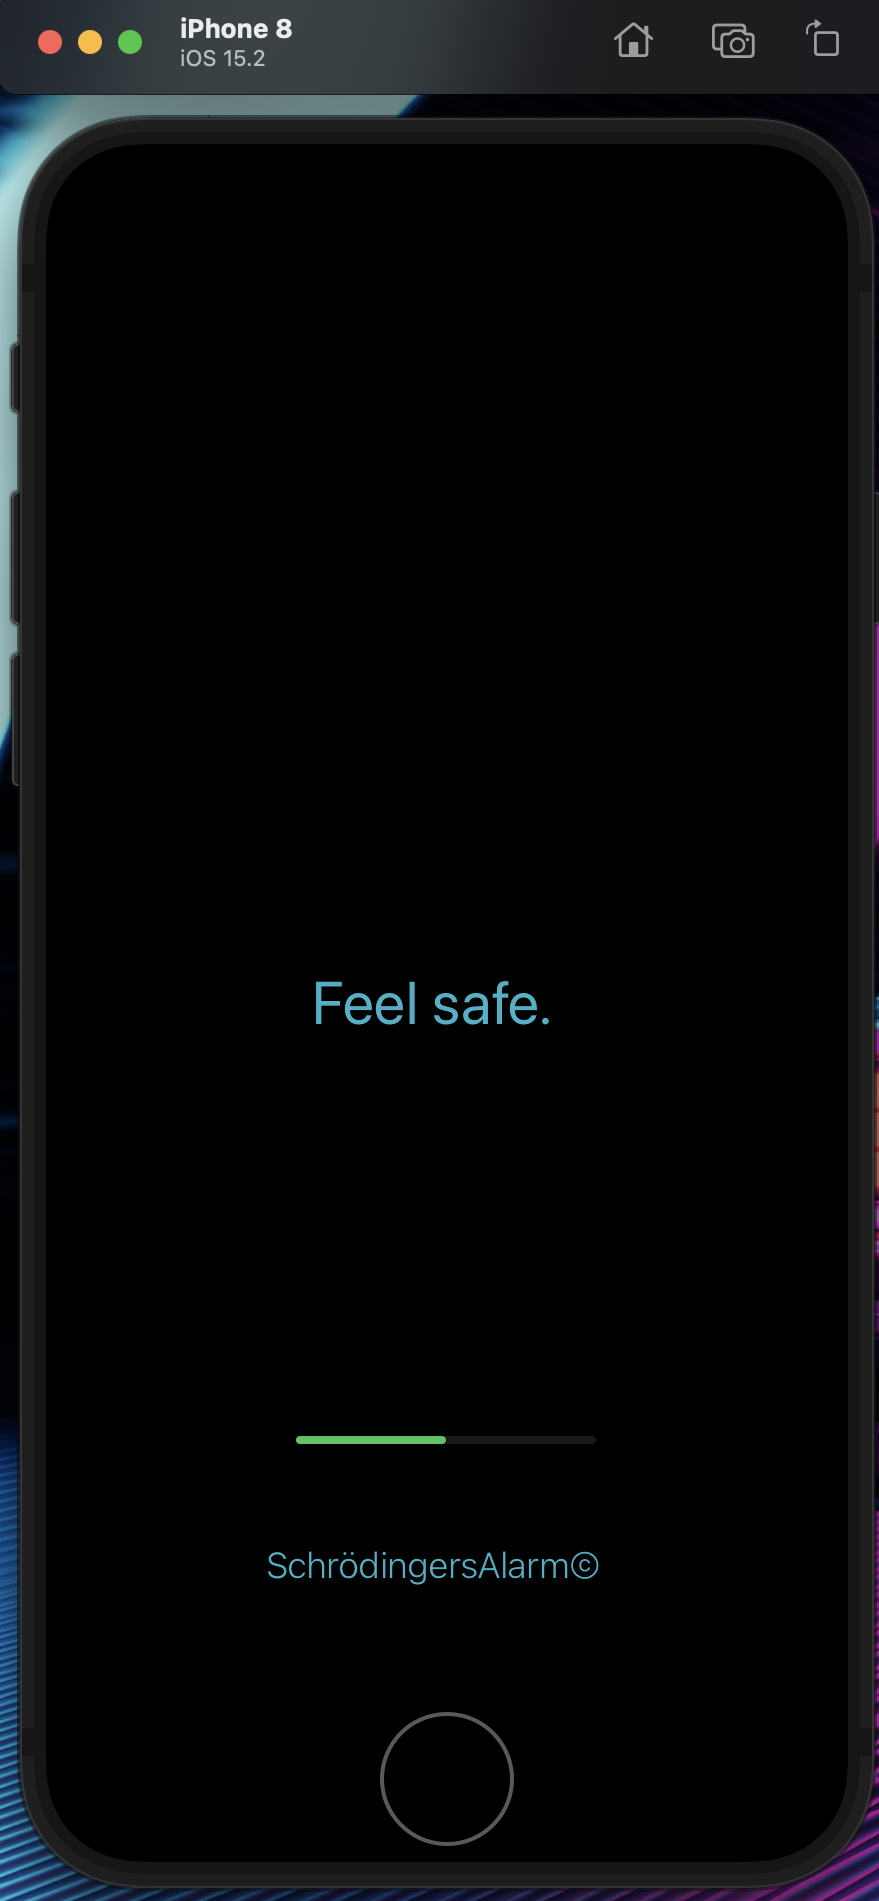
\includegraphics[width=0.4\textwidth]{Bilder/iOS_launch.png}
		\caption{Launchscreen}
		\label{Launch}
	\end{center}
\end{figure}
Beim Blick auf den Home-Bildschirm, im Navigations-Menü am kleinen Häuschen unten auf Daumenhöhe zu erkennen, sticht sofort das große Schloss ins Auge. Dieses kann auch wortwörtlich verstanden werden - ist es grün, dann ist der Alarm aktiviert \textit{(verschlossen, gesichert)}, tapt der Nutzer erneut darauf, ist es rot und der Alarm deaktiviert \textit{(geöffnet, ungesichert)}.
\begin{figure} [H]
	\begin{center}
		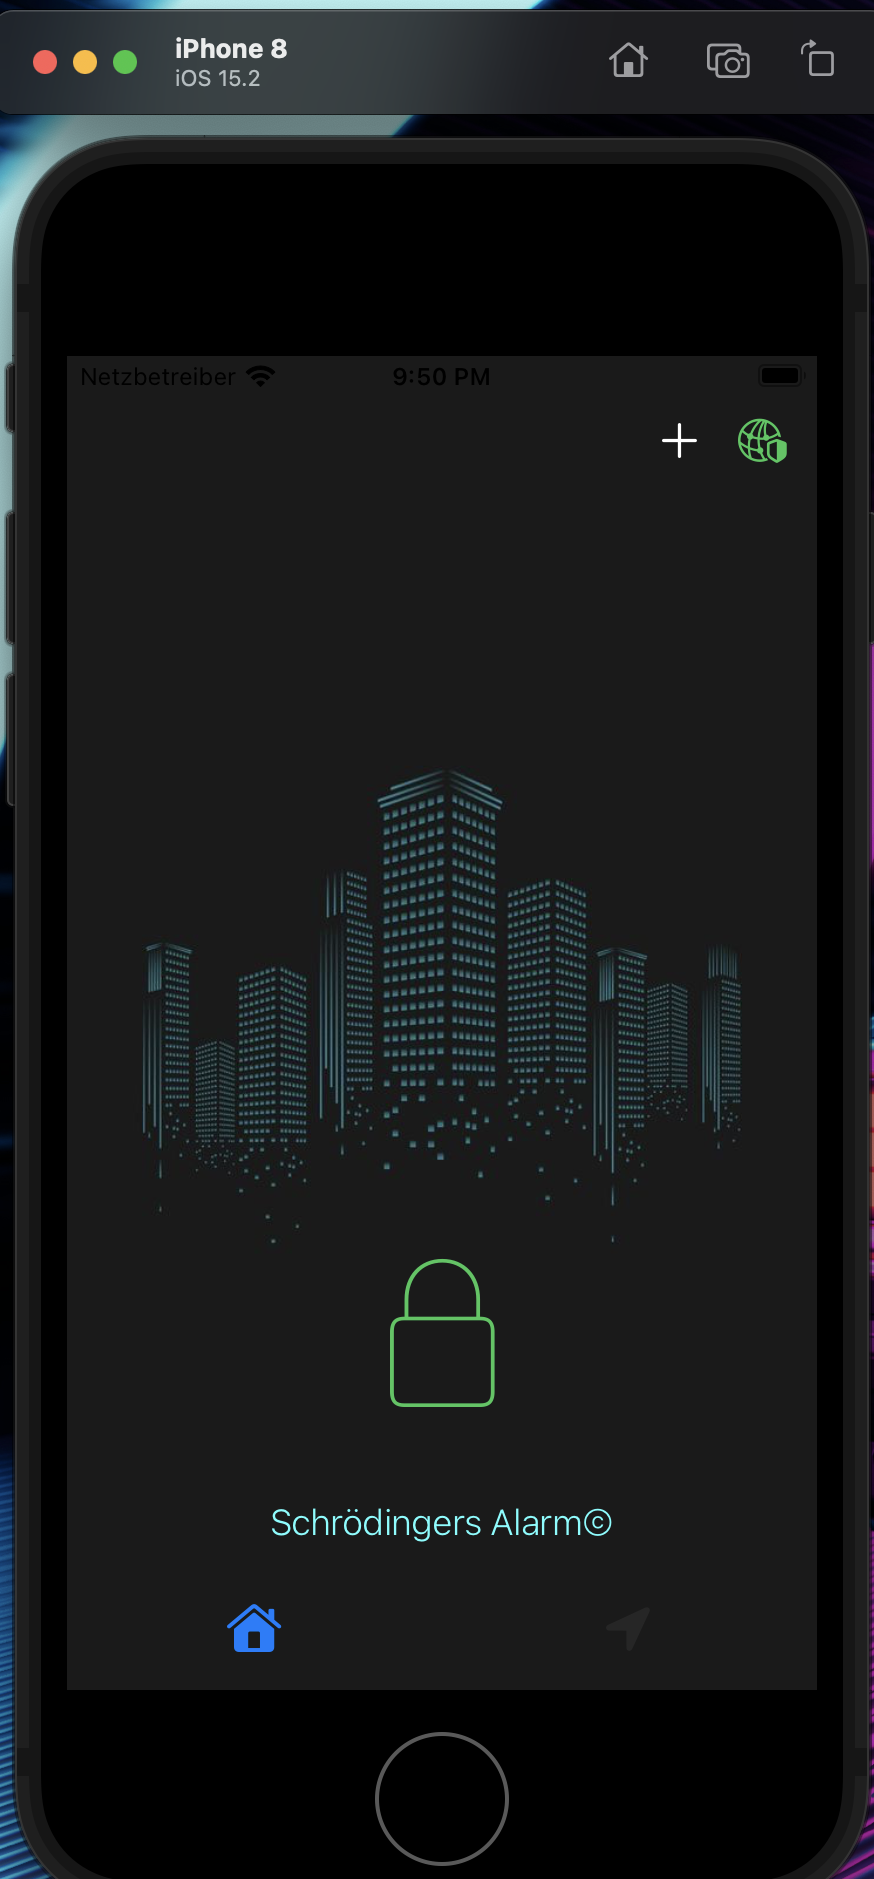
\includegraphics[width=045\textwidth]{Bilder/iOS_home.png}
		\caption{Navigationstab \textit{Home im aktivierten Modus}}
		\label{lock}
	\end{center}
\end{figure}
Bei der Umsetzung  des Kartendesigns war es wichtig, dass der Nutzer die vom Server bereitgestellten Daten angezeigt bekommt. Das  Feature, dass diese nicht als plain-Text dargestellt, sondern die Koordinaten direkt als Standort auf einer Karte übersetzt werden, haben wir ebenfalls umgesetzt, wie in Abbildung \ref{Map} visualisiert.
\begin{figure} [H]
	\begin{center}
		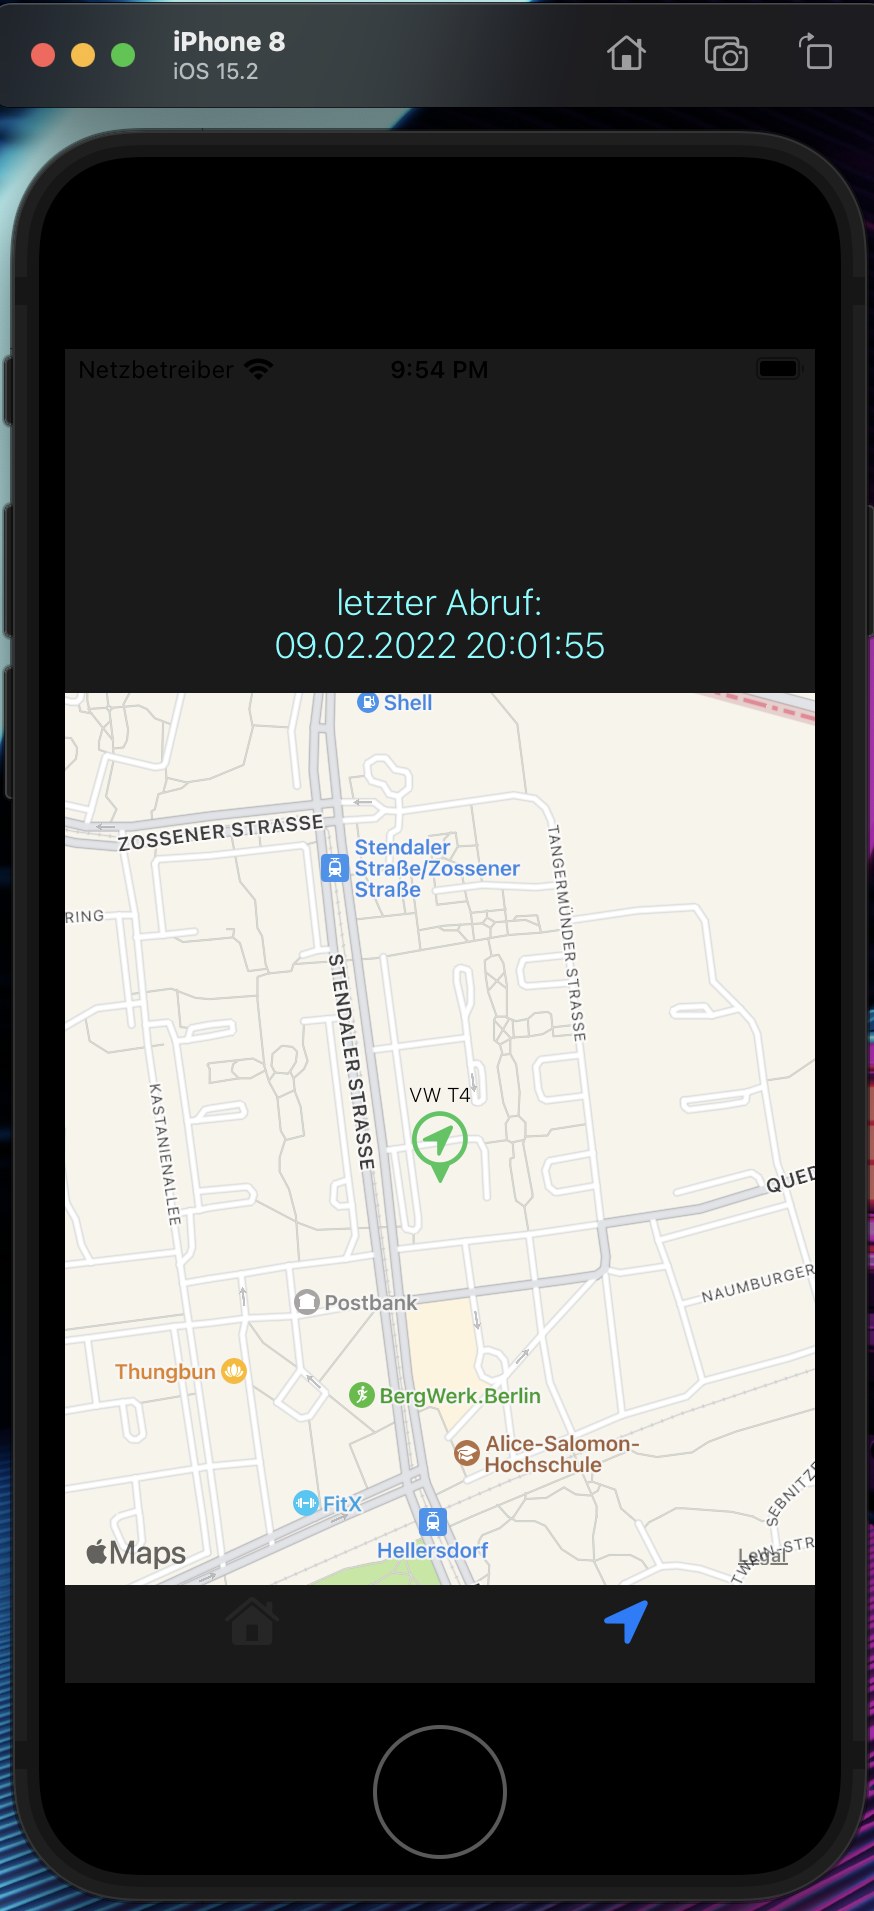
\includegraphics[width=0.4\textwidth]{Bilder/iOS_map.png}
		\caption{Navigationstab \textit{Map}}
		\label{Map}
	\end{center}
\end{figure}
Zur noch besseren Vorstellung, wie das Handling der beiden Apps ist, sind unter \textbf{Anhänge} die Links zu den jeweiligen auf Youtube hochgeladenen Demonstrations-Videos hinterlegt.



\subsection{Probleme}
Wie bereits angeteasert, gab es bei der Entwicklung einige Probleme, es waren kleinere wie anfänglich kein ausreichend leistungsstarkes und zudem mit aktuellem Betriebssystem ausgestattetem Macbook und größere, wie nachfolgend genauer beschrieben.
\\
\\
\subsubsection{Koordinaten in JSON als String hinterlegt}

Zu Beginn wurden die Koordinaten, sowie der Abrufzeitpunkt als Strings vom Server zur Verfügung gestellt, was ein Parsen sehr erschwerte, da für die Verarbeitung dieser Daten die iOS-Map integer beziehungsweise double-Werte benötigt. Dies Problem konnte jedoch nach interner Rücksprache schnell behoben werden, da es sich lediglich um eine Einstellung beim Encode des Webservers handelte.

\subsubsection{Http? Abrufen verboten!}

Die benötigten Daten vom Server werden nicht innerhalb der App angezeigt und es erweckte auch nie den Anschein, dass diese überhaupt abgerufen werden. Es wurde sehr lange das Problem innerhalb der Methoden gesucht, jedoch ohne nennenswerte Erkenntnisse. Erst als extern um Hilfe gebeten wurde, kam schnell heraus, dass SwiftUI den Abruf von JSON-Daten einer Http-Seite verhindert. Nach gezielter Platzierung von print()-Ausgaben im Log wurde das eigentliche Problem sichtbar, siehe Abbildung \ref{fehler}. Bei Nutzung einer Beispiel JSON-Datei von einer Https-Seite trat keine Fehlermeldung mehr auf.
\begin{figure} [H]
	\begin{center}
		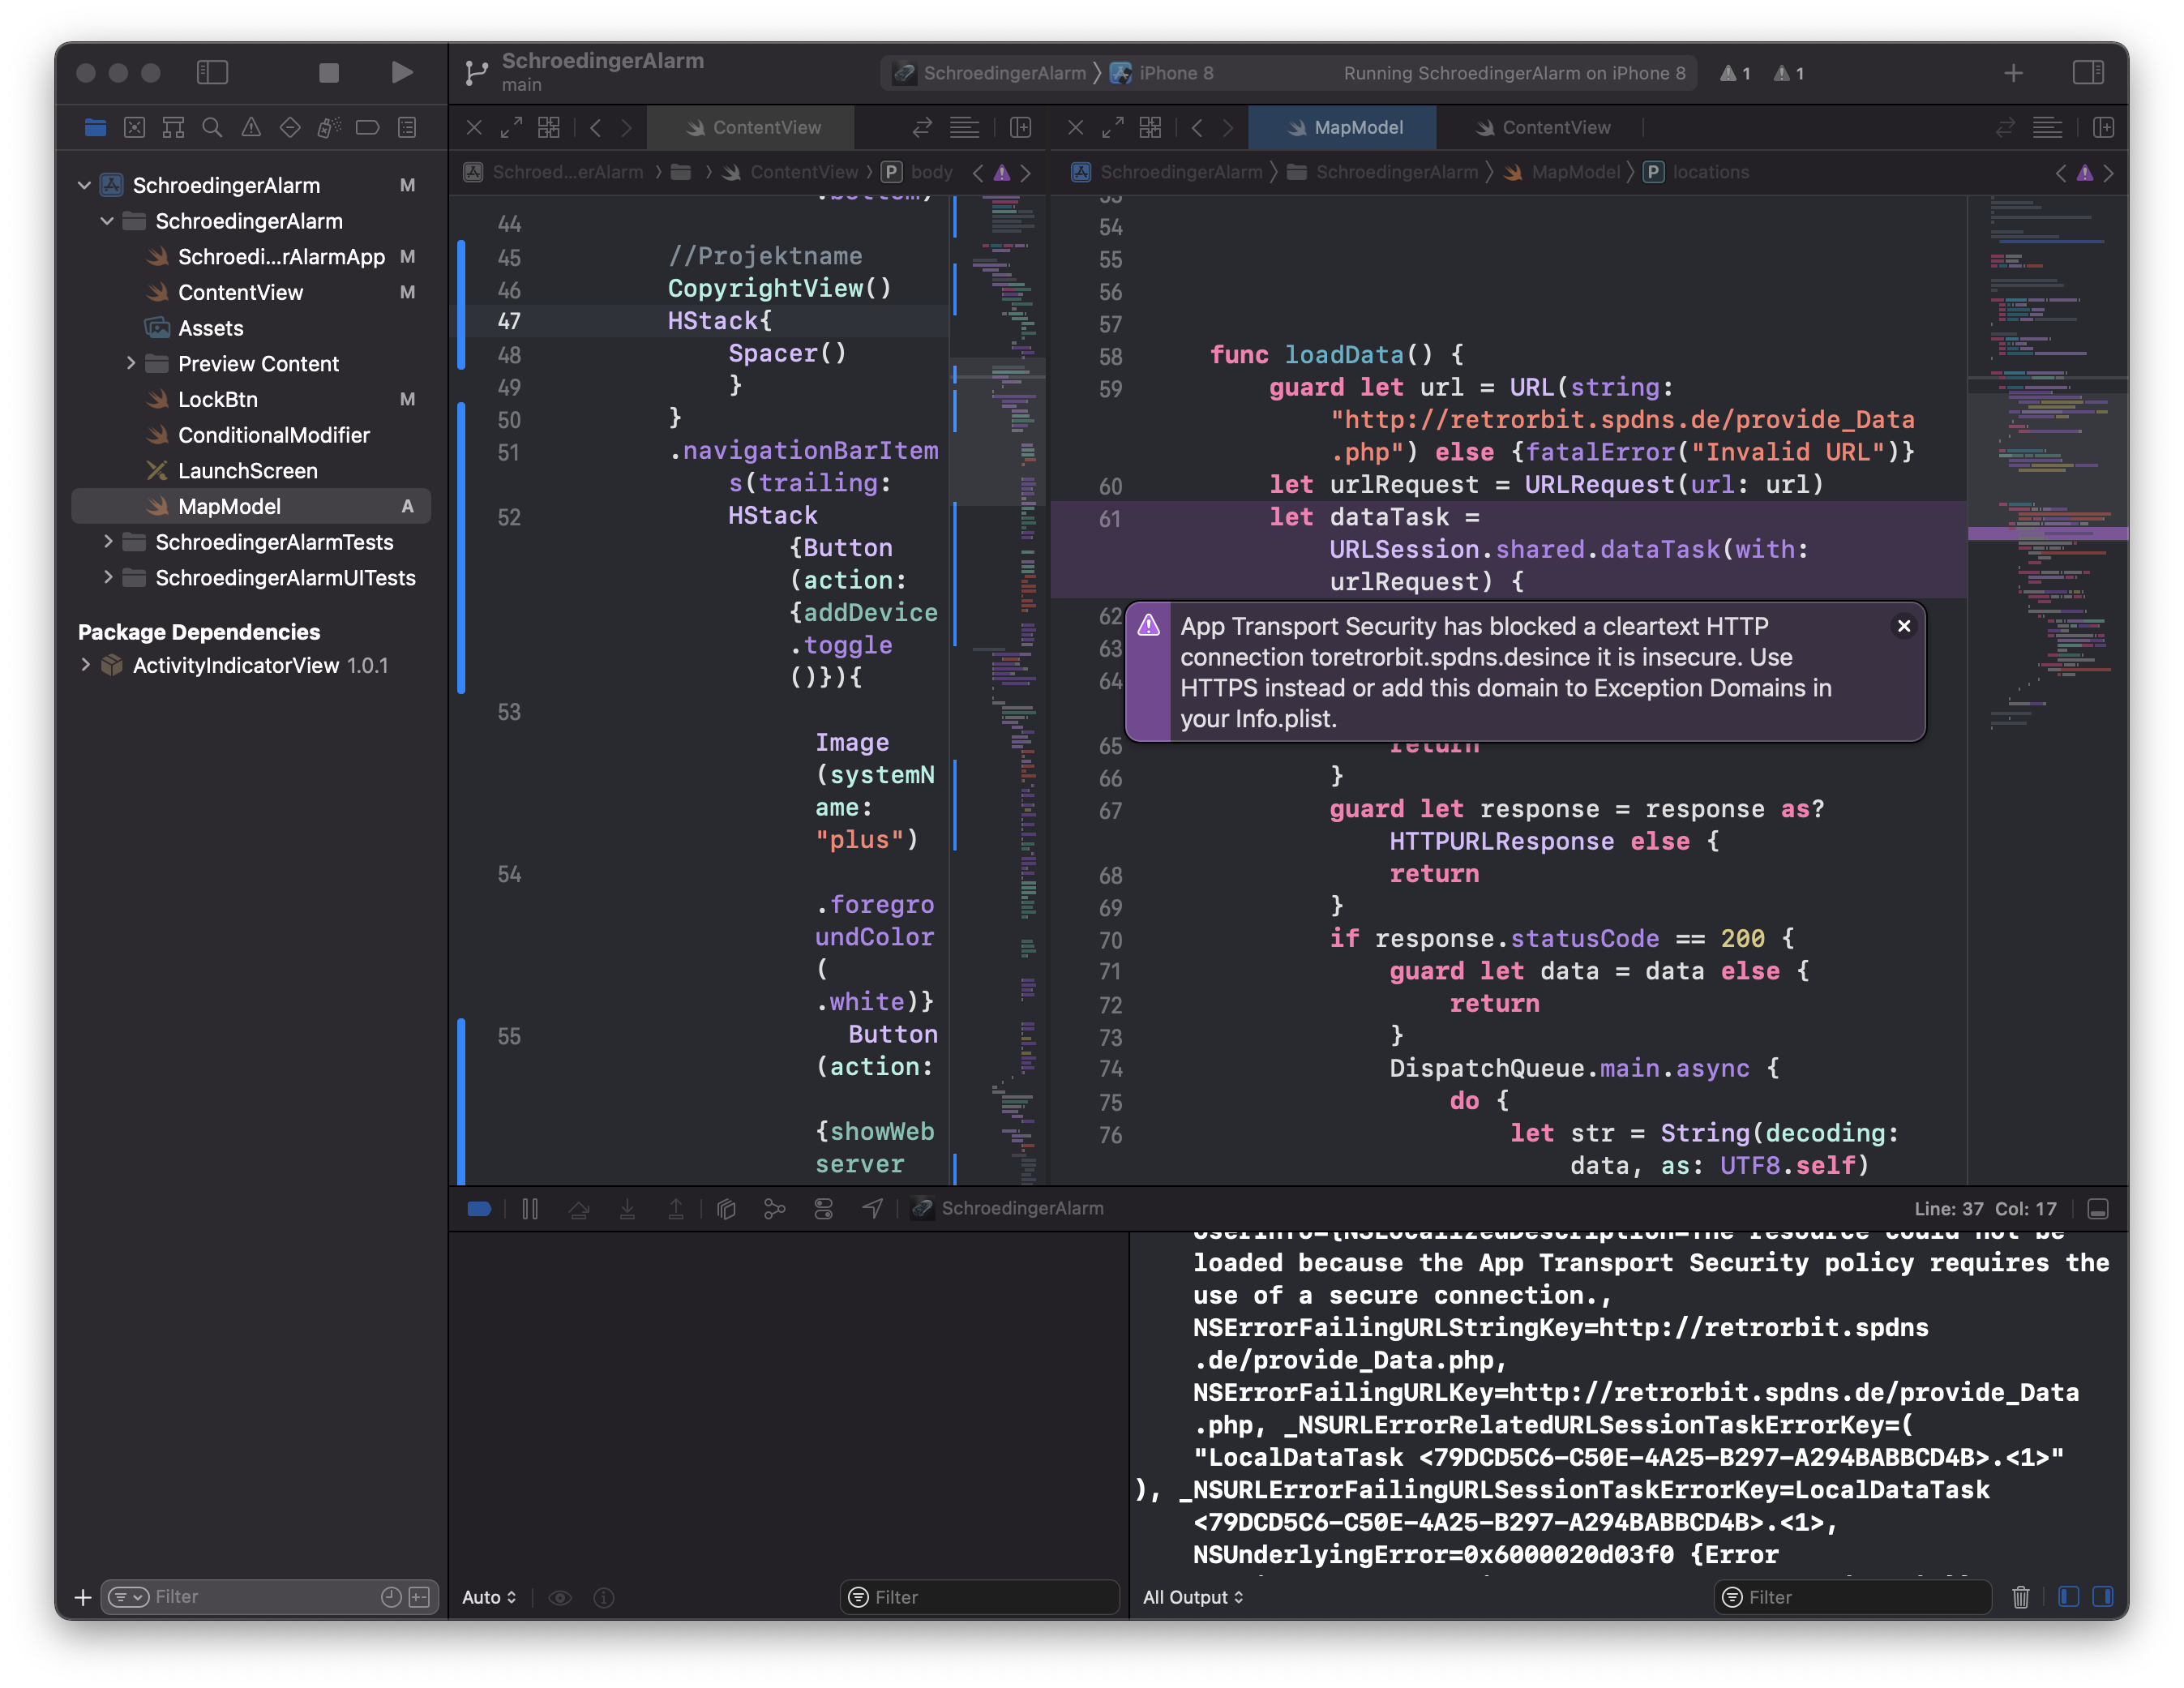
\includegraphics[width=1\textwidth]{Bilder/iOS_fehlermeldung.png}
		\caption{Fehlermeldung \textit{NSAppTransportSecurity}}
		\label{fehler}
	\end{center}
\end{figure}
Auf Apple-Plattformen verbessert eine Netzwerkfunktion namens App Transport Security (\textit{ATS}) den Datenschutz und die Datenintegrität für alle Apps und App-Erweiterungen. ATS erfordert, dass alle HTTP-Verbindungen, die mit dem URL-Ladesystem hergestellt werden – normalerweise unter Verwendung der URLSession-Klasse – HTTPS verwenden. Es erlegt außerdem erweiterte Sicherheitsprüfungen auf, die die vom TLS-Protokoll\footnote{Transport Layer Security} vorgeschriebene Standard-Server-Vertrauensbewertung ergänzen. ATS blockiert Verbindungen, die die Mindestsicherheitsanforderungen nicht erfüllen. [..] Diese Schutzmaßnahmen können umgangen werden, indem der NSAppTransportSecurity-Schlüssel zur Information Property List-Datei der App hinzugefügt und ein ATS-Konfigurationswörterbuch als Wert angegeben wird \cite{Inc}
\\
\\
Dieses Problem kann also behoben werden, wurde aber leider nicht mehr innerhalb der Bearbeitungszeit geschafft und wird später nachgeholt.